\documentclass[skripta, fancy]{FSBtex}

\graphicspath{{./slike}}

\usepackage{lipsum}

% naredbe za generiranje datoteke
% pdflatex main.tex
% bibtex main
% makeindex -s nomencl.ist -o main.nls main.nlo
% makeglossaries-lite main
% pdflatex main.tex
% pdflatex main.tex



\Author{Marko Markić}

\TitleHR{Skripta}


%%%%%%%%%%%%%%
% za titlefancyfigure opciju slika svakog poglavlja
%%%%%%%%%%%%%%
% sve opcije se mogu mijenjati za zvako poglavlje pozivanje pojedine opcije
%\chapterimage{naslovna1.jpg} % slika poglavlja
%\chapterspaceabove{6.5cm} % razmak od vrha stranice do naslova poglavlja
%\chapterspacebelow{6.75cm} % razmag ot gornje margine do pocetka teksta

%----------------------------------------------------------------------------------------
%	POCETAK DOKUMENTA
%----------------------------------------------------------------------------------------
\begin{document}
\titlepage	% ova naredba ukljucuje sve naslovne strane rada ovisno o tipu rada, te sadrzaj i popise slika i tablica

% sve sa A se prvo ispisuje kod oznaka
\nomenclature[A]{$s$}{klizna površina SMC regulatora \nomunit{\si{\kilogram\per\cubic\meter}}}
\nomenclature[A]{$k_1,\ k_2$}{pojačanja SMC regulatora \nomunit{-}}%
\nomenclature[A]{$k_1,\ k_2,\ k_3$}{pojačanja metode povratnog koraka \nomunit{-}}%

% konstante
\nomenclature[C]{$g$}{gravitacijsko ubrzanje  \nomunit{9,81 \si{\meter\per\square\second}}}%

%% grcke oznake
\nomenclature[G]{$\beta,\ \gamma$}{težinski koeficijenti PID regulatora \nomunit{-}}%
\nomenclature[G]{$\rho$}{gustoća fluida, \nomunit{\si{\kilogram\per\cubic\meter}} }%

% indeksi
\nomenclature[I]{$\alpha_d$}{koeficijent istjecanja \nomunit{-}}%

% akcenti
\nomenclature[T]{$\underline{\square}$}{Dual quaternion }%

% kratice
\newacronym{iot}{IoT}{internet stvari (eng. \textit{Internet of Things})}
\newacronym{lqri}{LQR-I}{linearni kvadratični regulator s integralnim djelovanjem}
% vidi poglavlje 2 za primjenu
  
 
%----------------------------------------------------------------------------------------
%	OVDJE IDE OSTATAK RADA I SVA POGLAVLJA
%----------------------------------------------------------------------------------------

% pocetak brojanja rada od prve stranice
\PageNumberingArabic

%\chapterimage{naslovna2.jpg}
%\chapterspaceabove{5.5cm}
\chapter{Quaternions \& dual quaternions dasf dsaf das fads fads fadsf agd a}
\lipsum[1-1]

\begin{figure}[h!]
\centering
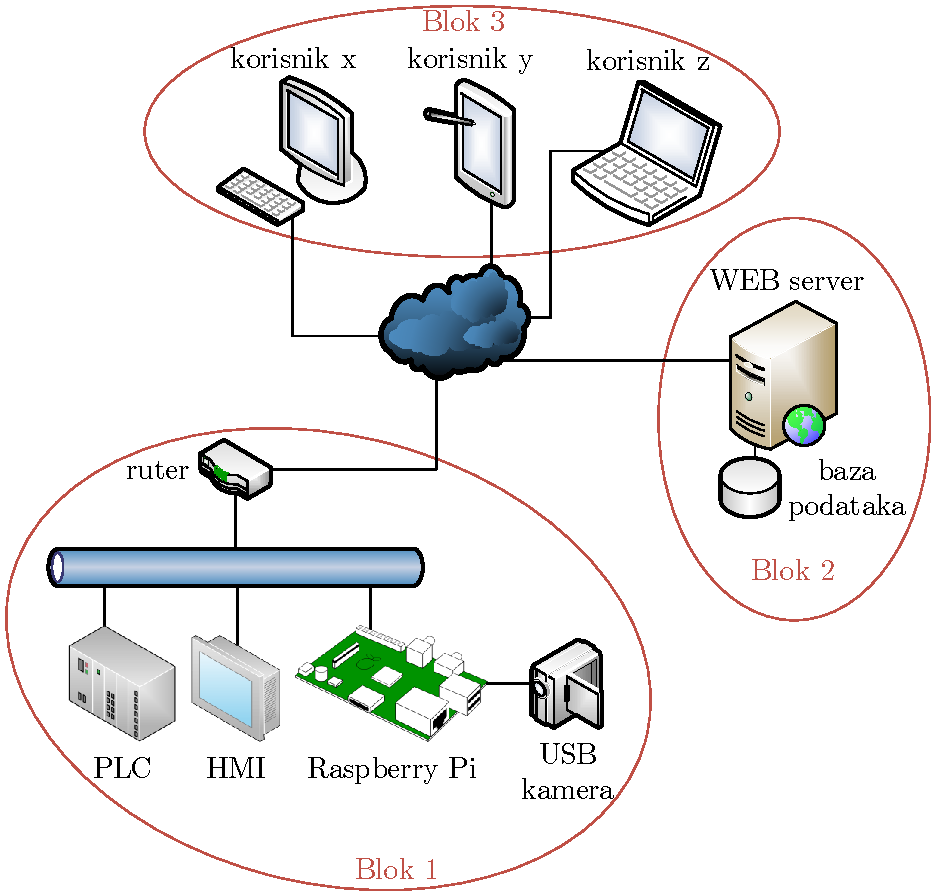
\includegraphics[scale=.5]{IoT_ideja.pdf}
\caption{Proba slika}
\end{figure}

\lipsum[1-1]

\begin{theorem}[Proba]
asdfdsa fsda fdasf dfkaj akijf eoaif
\begin{equation}
c^2 = a^2+b^2ˇ
\end{equation}
\end{theorem}

\lipsum[1-2]
\acrlong{lqri}
\begin{definition}[Proba]
asdfdsa fsda fdasf dfkaj akijf eoaif
\begin{equation}
c^2 = a^2+b^2ˇ
\end{equation}
\end{definition}

\begin{remark}
adsfds fads fasd 
\end{remark}

\lipsum[1-2]


\begin{proof}[adsf]
a = b
\end{proof}

\begin{exercise}
sdfo dks fodkas fladskf pšasd
\begin{equation}
a = c\cdot b
\end{equation}
\end{exercise}


\begin{example}[Primjer sadf]
sdfo dks fodkas fladskf pšasd
\begin{equation}
a = c\cdot b
\end{equation}
\end{example}




\chapter{Test Chapter Two}
\acrlong{iot} \cite{dq_fkm_control}
\section{Second section} 
\subsection{dsfdasf}
\subsubsection{sdafdas}
\acrshort{iot}
\lipsum[5-8]



% literatura:
\LiteratureSettings
\bibliography{literatura}


\appendix
\chapter{Prilog matematička notacija}
\section{poadsfkj opdska f}


\end{document}





